\documentclass[11pt]{article}
\usepackage{amsthm}
\usepackage{amsmath}
\usepackage{amssymb}
\usepackage{ifthen}

\usepackage{graphicx}
\graphicspath{ {./images/} }

\let\oldcite=\cite
\renewcommand\cite[1]{\ifthenelse{\equal{#1}{NEEDED}}{[citation~needed]}{\oldcite{#1}}}

\title{How effective are passwords as a means of authentication, how can they be attacked and how can they be made more resilient to attack?}
\author{Lucian James}

\begin{document}
\maketitle
\begin{abstract}
The aim of this project is to determine the strengths and weaknesses of using passwords as a means of authentication, primarily for online accounts.
Protocols for password authentication will be introduced, at various levels of complexity and security.
Attacks that can take place against these protocols will then be detailed, then the methods which can be used to secure systems against these attacks.
\end{abstract}

\section{Introduction} \label{INTRO}
Passwords have been used to verify identity since ancient times\cite{NEEDED}.
In the modern world passwords are used primarily for login processes for computer devices and online services. 
A typical computer user will use passwords for many different purposes ranging from accessing their computer to performing online bank transactions.
Due to the high importance that the confidentiality, integrity and availability of our data is maintained, it is of great importance that the procedures we use to verify identity in order to allow access to our data are highly secure.
This project will assess the role that passwords play in modern authentication, and the issues surrounding the use of passwords, both the technical and human aspects will be considered.
The primary issue with password-based authentication is that it relies on only one authentication factor; `Something the user knows', this can be problematic as knowledge factors can be obtained by attackers sometimes with ease compared to other factors, such as "Something the user has" or "Something the user is".
The fact that password authentication relies only on a knowledge factor does make it very convenient for users, as there is no requirement for additional hardware or software to authenticate with a system (such as fingerprint scanners or smartcards).
The primary cause of concern around the use of knowledge factors is that users may choose an easily guessed piece of knowledge, or fail to maintain the secrecy of the knowledge, which can cause great insecurity towards their accounts and thus their data.
This project will focus primarily on authentication to online servers across a network assumed to be unsafe, but some mention of other use cases will (probably) be made.\\



\section{Password protocols} \label{PP}
Protocols are a system of rules and/or procedures that define how two entities interact. A password protocol is then to no surprise, a system of rules and/or procedures that define how authentication using a password takes place.
The basic goal of almost all password protocols is simple; Allowing one party to prove that it knows some password, usually set in advance. Protocols which achieve this range from the trivial to the incredibly complex \cite{wu1998secure}.
This section is important as developing an understanding of the various levels of security different protocols provide will be important for section \ref{VULN}.

\subsection{A basic password authentication protocol (PAP)} \label{PAP}
In the simplest form of a password authentication protocol, the user/client sends to the host/server their plaintext username and password, then the server verifies the password either by comparing it directly to a stored plaintext password or applying a one-way hash function to the received password and comparing it to a stored hash. 
Since the users plaintext password is immediately exposed to being intercepted, this method is unacceptable for use on untrusted networks.
Such a protocol is described in IETF RFC1334 \cite{simpson1992pap}:
\begin{quote}
``The Password Authentication Protocol (PAP) provides a simple method for the peer to establish its identity using a 2-way handshake. 
This is done only upon initial link establishment.\\
After the Link Establishment phase is complete, an Id/Password pair is repeatedly sent by the peer to the authenticator until authentication is acknowledged or the connection is terminated.\\
PAP is not a strong authentication method. 
Passwords are sent over the circuit `in the clear', and there is no protection from playback or repeated trial and error attacks. The peer is in control of the frequency and timing of the attempts''
\end{quote}

\subsection{Challenge handshake authentication protocol (CHAP)} \label{CHAP}
IETF RFC1994 \cite{simpson1996chap} details a protocol for authentication which provides protection against playback attacks, as the password is not communicated across the connection between the client and the server.
The mechanism of the challenge handshake authentication protocol is described as so:
\begin{enumerate}
\item User sends their identity to the server.
\item The server uses the identity received from the user to fetch the required information, such as its copy of the users password ($p_{server}$).
\item The server sends the user a random message, known as a challenge ($c$).
\item The user uses some hashing function ($h$) to generate a response ($r$) to the challenge, using their password ($p_{user}$) and the random message received from the server. $r = h(p_{user},c)$
\item The user then sends $r$ to the server.
\item The server makes a comparison, if $r = h(p_{server},c)$ then the user is authenticated, because $h(p_{user},c) = h(p_{server},c) \Longrightarrow p_{user} = p_{server}$.
\item At random intervals after successful authentication has taken place, the server sends new challenges to the user, repeating the above steps.
\end{enumerate}
Since $h(p_{user},c)$ is sent across the network in this verification process instead of the plaintext password and $c$ is unique for every authentication, interception is a less viable attack.
Although if $r$ and $c$ are captured by an attacker and $h$ is a known function, the attacker can attempt to find the value of $p_{user}$ by calculating $h(x,c)$ and comparing it with $r$, where $x$ is an arbitrary guess at what the password could be.
$$h(x,c)=r \Longrightarrow x = p_{user}$$
The process can be repeated as many times as required with different values of $x$ to find the value of $p_{user}$. As passwords are often considered low-entropy secrets \cite{NEEDED}, the ability for an attacker to perform offline attacks in unacceptable.
Another issue with CHAP is that passwords are stored as plaintext on the server, irreversible encryption (hashing) cannot be used. If an attacker captures the password files they can use them to authenticate with the server with ease.

\subsection{General encryption protocols} \label{GEP}
One option to ensure security of authentication is to encrypt all communications using some form of asymmetric encryption.
An example of a protocol which allows for this kind of encryption is the Transport Layer Security (TLS) protocol, which is utilised by HTTPS.
TLS is most likely the most commonly used method of securing communications, including of course communications during authentication.
When all communications are encrypted very simplistic protocols such as PAP can be used, as interception is prevented by the encryption of the communications.\\\\
The almost universal method of authentication utilises TLS for security, and can be outlined as so:
\begin{enumerate}
\item A client-to-server TLS channel is established.
\item The client sends their identity and password $p_{user}$ through the TLS channel.
\item The server runs the password received from the client through a hash function $h$. 
\item The server compares $h(p_{user})$ with its stored hash of the correct password $h(p_{server})$. $$h(p_{user}) = h(p_{server}) \Longrightarrow p_{user} = p_{server}$$
\end{enumerate}
Using a secure communication protocol greatly reduces the need for a secure authentication protocol, but it does come with its disadvantages, these include:
\begin{enumerate}
\item The password appears in plaintext at the server during authentication. This can be a problem as this information could me mistakenly logged and stored on the server. This has occurred on the servers of even the biggest websites in the world. It has been reported that both twitter\cite{heeti2018twitter} and facebook\cite{whittaker2019facebook} have mistakenly stored plaintext passwords in the past.
\item Public-key infrastructure failures can occur which causes the security to be compromised, these can include:
\begin{itemize}
\item Theft of server private keys.
\item Software that does not verify certificates correctly.
\item Users that accept invalid or suspicious certificates.
\item Certificates issued by rogue certificate authorities.
\item Servers that share their TLS keys with others - e.g., CDN providers or security monitoring software.
\item Information (including passwords) that traverses networks in plaintext form after TLS termination
\item And more! :)
\end{itemize}
\end{enumerate}
\cite{jarecki2018opaque}

\subsection{Password-authenticated key exchange (PAKE)} \label{PAKE}
Password-authenticated key exchange protocols provide a method for two parties to establish a shared key based on their shared knowledge of a secret password, in a way which is immune to offline attacks \cite{jarecki2018opaque}.
PAKE can be used to provide secure authentication without the issues listed in section \ref{GEP}, as well as protection against other attacks such as man-in-the-middle attacks.

\subsubsection{The secure remote password protocol} \label{SRP}
A PAKE protocol of note is the ``Secure Remote Password Protocol'' (SRP protocol), designed in 1998 \cite{wu1998secure}.
The mechanism of the 1998 original version of the SRP protocol can be described as so:\\
Password establishment:
\begin{enumerate}
\item To establish a password $P_1$ with the server, the client picks a random salt $s$ and computes $x_1=H(s,P_1)$, where $H$ is some hash function. As well as $v=g^{x_1}$, where $g$ is a primitive root modulo $n$ (often called a generator) where $n$ is a large prime number. The values $g$ and $n$ and well-known and agreed beforehand.
\item The server then stores $v$ and $s$ as the clients password verifier and salt. $x_1$ is discarded because it is equivalent to the plaintext password $P$.
\end{enumerate}
Authentication:
\begin{enumerate}
\item The client sends the server its username.
\item The server looks up the users password entry and fetches the users password verifier $v$ and the users salt $s$. The server sends $s$ to the client. The client then computes its long-term private key $x_2$ using $s$ and the password $P_2$. $x_2=H(s,P_2)$ where $H$ is some hash function.
\item The client generates a random number $a$, $1<a<n$, and computes its ephemeral public key $A=g^a$, and sends it to the server.
\item The server generates a random number $b$, $1<b<n$, and computes its ephemeral public key $B=v+g^b$, and sends it back to the client, along with a randomly generated parameter $u$.
\item The client computes $S_1=(B-g^{x_2})^{a+ux_2}$, and the server computes $S_2=(Av^u)^b$. 
$P_1=P_2 \Longrightarrow S_1=S_2$, which means that if both the client and the server get the same value of $S$ then the client has the correct password.
\begin{proof}[Proof $P_1=P_2 \Longrightarrow S_1=S_2$]
\begin{align*}
S_2&=(Av^u)^b\\
&=(g^a((g^{H(s,P_1)})^u))^b\\
&=(g^a(g^{u(H(s,P_1))}))^b\\
&=(g^{a+u(H(s,P_1))})^b\\
&=g^{b(a+u(H(s,P_1)))}\\
&=g^{ba+bu(H(S,P_1))}
\end{align*}
\begin{align*}
S_1&=(B-g^{x_2})^{a+ux_2}\\
&=(g^{H(s,P_1)}+g^b-g^{H(s,P_2)})^{a+u(H(s,P_2))}
\end{align*}
\begin{align*}
P_1=P_2 \Longrightarrow g^{H(s,P_1)}-g^{H(s,P_2)}=0\\
\therefore (g^{H(s,P_1)}+g^b-g^{H(s,P_2)})^{a+u(H(s,P_2))}&=(g^b)^{a+u(H(s,P_2))}\\
&=g^{b(a+u(H(S,P_2)))}\\
&=g^{ba+bu(H(S,P_2))}
\end{align*}
$$P_1=P_2 \Longrightarrow g^{ba+bu(H(S,P_2))}=g^{ba+bu(H(S,P_1))} \therefore S_1=S_2$$
\end{proof}
\item Using some hash function $H$, the client computes $K_1=H(S_1)$ and the server computes $K_2=H(S_2)$. $K$ is a cryptographically strong session key.
\item The client uses some hash function $H$ to calculate $M_1=H(A,B,K_1)$.
\item The client sends the server $M_1$ as evidence that it has the correct session key. The server then computes $M_1$ itself and verifies that it matches what the client sent.
\item The server calculates $M_2=H(A,M_1,K_2)$.
\item The server sends the client $M_2$ as evidence that it also has the correct session key, The client also verifies $M_2$ itself, accepting only if it matches the value the server provided.
\end{enumerate}
The SRP protocol has the following advantages:
\begin{itemize}
\item If the hosts password file is captured and the intruder learns the value of $v$, it should still not allow the intruder to impersonate the user without an expensive dictionary search to find the value of $P_1$.
\item Unlike earlier PAKE protocols, it does not require the passwords to be stored on the server in plaintext, instead, the server stores a ``verifier'' which is a one-way function of the the password hash. This means that a breach of the database does not immediately allow an attacker to impersonate users, they must first perform expensive dictionary attacks to obtain the raw passwords. The technical name for this is asymmetric password-authenticated key exchange.
\item Public-key infrastructure is not required.
\item Despite drawbacks that it may have, the SRP protocol is simple, there is working code in OpenSSL that even integrates with TLS, which makes it relatively easy to adopt.
\end{itemize}
The SRP protocol has the following disadvantages:
\begin{itemize}
\item Earlier versions of the SRP protocol have been broken several times, which is why the protocol is currently on revision 6a. Additionally the ``security proof'' in the original paper doesnt really prove anything meaningful.
\item The SRP protocol leaks salt to unknown users by design, making it vulnerable to pre-computation attacks.%(DESCRIBE WHAT PRECOMPUTATION ATTACK IS)
\end{itemize}
\cite{green2018pake}

\subsubsection{OPAQUE}
A more recent PAKE protocol of note is ``OPAQUE'', which is an asymmetric PAKE protocol secure against pre-computation attacks \cite{jarecki2018opaque}.
A description of the full mechanism of this protocol is out of the scope of this project (The paper is 61 pages long!), but the benefits which it offers over a protocol such as the SRP protocol can be described easily thanks to \cite{green2018pake}:
\begin{itemize}
\item OPAQUE does not reveal salts to potential attackers. This is done by combining the salt with the password, in a way which ensures the client does not learn the salt and the server does not learn the password.
\item OPAQUE works with any password hashing function.
\item All the hashing work is done on the client, which means OPAQUE can actually take load off the server.
\item Unlike SRP, OPAQUE has a reasonable security proof.
\end{itemize}
\cite{green2018pake}
\begin{center}
\textbf{Details about salt secrecy}\\
\end{center}
``The main problem with earlier PAKEs is the need to transmit the salt from a server to a (so far unauthenticated) client. This enables an attacker to run pre-computation attacks, where they can build an offline dictionary based on this salt.''\\\\
``The challenge here is that the salt is typically fed into a hash function (like scrypt) along with the password. Intuitively someone has to compute that function. If it’s the server, then the server needs to see the password — which defeats the whole purpose. If it’s the client, then the client needs the salt.''\\\\
``OPAQUE gets around this with the following clever trick. They leave the password hash on the client’s side, but they don’t feed it the stored salt. Instead, they use a special two-party protocol called an oblivious PRF\footnote{Pseudo Random Function} to calculate a second salt (call it salt2) so that the client can use salt2 in the hash function — but does not learn the original salt.
The basic idea of such a function is that the server and client can jointly compute a function PRF(salt, password), where the server knows `salt' and the client knows `password'. Only the client learns the output of this function. Neither party learns anything about the other party’s input.''\cite{green2018pake}\\\\
The implementation of oblivious PRF relies on the idea that the client has the password $P$ and the server has the salt $s$.
The output of the PRF function should be in the form $H(P)^s$ where $H$ is a special hash function that hashes passwords into elements of a cyclic (prime-order) group.\\\\
To compute this, PRF requires a protocol between the client and server. In this protocol, the client first computes $H(P)$ and then `blinds' this password by selecting a random scalar value $r$, and blinding the result to obtain $C=H(P)^r$. At this point, the client can send the blinded value $C$ over the server, secure in the understanding that (in a prime-order group), the blinding by $r$ hides all partial information about $P$.\\\\
The server, which has salt value $s$, now further exponentiates this value to obtain $R=C^s$ and sends $R$ back to the client. Written out in detail, the result can be expressed as $R=H(P)^{rs}$. The client now computes the inverse of its own blinding value $r$ and exponentiates one more time as follows: $R'=R^{r^-1}=H(P)^s$. This element $R'$, which consists of the hash of the password exponentiated by the salt, is the output of the desired PRF function.\\\\
A nice feature of this protocol is that if the client enters the wrong password into the protocol, it should obtain a value which is very different from the actual value it wants. This guarantee comes from the fact the hash function is very likely to produce wildly different outputs for distinct passwords.\\\\
Theoretically, the salt can be found. The client knows the value of $R'$ which is equal to $H(P)^s$, and the value of $H(P)$, so theoretically it is possible to find the value of $s$ by computing $log_{H(S)}R'$. But this is only a theoretical possibility, as under the condition that the value produced by $H(P)$ is $2q+1$ where $q$ is a large prime number, this calculation falls into the discrete logarithm problem, which is well known to be impractical to compute \cite{dong2016math}. 



\section{Password dataset and cracking analysis}
Might make sense for this to be its own section, despite the fact some individual parts fit may better into the vulnerabilities section.
\subsection{Datasets used} \label{datasets}
\begin{itemize}
\item \textbf{Top2Billion-probable-v2}\\
20.6gb file containing 1973218846 ``passwords'', they are ordered in the file starting with the most common to the least common. All items in this dataset are sourced from other datasets.\\
Sourced from the torrent listed on github.com/berzerk0/Probable-Wordlists.
\item \textbf{hk-hlm-founds.txt}\\
389.4mb file containing 38647798 ``passwords'', quick examination of the file shows some reasonably likely passwords and some gibberish.\\
Sourced from weakpass.
\item \textbf{cyclone.hashesorg.hashkiller.combined}\\
15.0gb file containing 1469156570 ``passwords'', quick examination of the file shows some reasonably likely passwords and some gibberish.\\
Sourced from weakpass.
\item \textbf{weakpass-3p}\\
14.5gb file containing 1454086314 ``passwords'', the file appears to be sorted alphabetically. fair amount of gibberish.\\
Sourced from weakpass.
\item \textbf{ASLM}\\
479.8mb file containing 41591035 ``passwords''.\\
Sourced from weakpass.
\item \textbf{pwned-passwords-ntlm-ordered-by-hash-v7}\\
20.6gb file containing 613584246 NTLM hashes of ``passwords'', along with the frequency that they are found in ``data breaches''.\\
Sourced from haveibeenpwned.
\item \textbf{Rules1.txt}\\
A set of rules for use during rule-based password cracking. It consists of 229 rules which modify input password guesses.
Sourced from weakpass with minor modification.
\end{itemize}
\subsection{Software used}
\begin{itemize}
\item C++ (g++ compiler)
\item Python
\item Hashcat
\end{itemize}
\subsection{Hardware used}
\begin{itemize}
\item CPU: AMD Ryzen 5 2600
\item RAM: 16GB
\item GPU: Nvidia Quadro P5000
\end{itemize}
\subsection{Dataset analysis}
\cite{pearman2017let} contains information about 4057 passwords (1522 unique) from 154 participants across 2077 web domains.
This paper provides a reliable real-world analysis to compare the password dictionaries I have collected to.
The characteristics of the data collected for this paper are as follows:
\begin{quote}
``On average, participants submitted a password 1.40 times per day. Including all passwords, participants had an average password length of 9.92 characters with their average password composed from 2.77 character classes including 2.70 digits, 5.91 lowercase letters, 0.84 uppercase letters, and 0.46 special characters.''
\end{quote}
Making a comparison between this information, and a similar analysis of the password dictionaries listed in \ref{datasets} provides some indication of how realistic these dictionaries are.
\begin{center}
\resizebox{\textwidth}{!}{%
\begin{tabular}{|p{5cm}|p{2cm}|p{3cm}|p{3cm}|p{2cm}|p{3cm}|}
 \hline
 Dataset & Avg length & Avg n uppercase & Avg n lowercase & Avg n digits & Avg n special \\ [0.5ex] 
 \hline\hline
 Top2Billion-probable & 10.01 & 0.969 & 5.8 & 3.14 & 0.174 \\
 \hline
 hk-hlm-founds & 9.56 & 0.715 & 5.49 & 3.26 & 0.386 \\
 \hline
 CHHC & 9.84 & 0.677 & 5.58 & 3.41 & 0.597 \\
 \hline
 weakpass-3p & 9.69 & 0.769 & 5.57 & 3.35 & 0.00 \\
 \hline
 ASLM & 11.1 & 0.23 & 5.47 & 4.34 & 5.40 \\
 \hline
\end{tabular}
}
\end{center}


\subsection{Password cracking analysis}

\subsubsection{Introduction}
Hashcat is a GPU-accelerated tool for cracking password hashes, it supports a wide range of hash types and many different attack modes.
This analysis will focus on dictionary attacks, with and without modification rules.
A dictionary attack is a method of discovering the correct password by systematically trying all entries in a ``dictionary''.
The ``correct'' password is the password which when sent through some hashing algorithm, produces an identical hash to the one which we are trying to decrypt.\\\\
Time taken is not considered in this analysis, as it varies greatly with the hardware being used, and the hashing algorithm used.
Instead, this analysis focuses on the number of passwords cracked from a set of hashes.\\\\
Modification rules can be used to augment a password dictionary by doing simple operations such as appending numbers, capitalising the first letter, etc.
For this analysis, the ``rules'' file consisted of 229 rules which perform simple modifications to every item in the input password dictionary, these modifications include, among others:
\begin{itemize}
\item Capitalising the first letter of passwords
\item Appending numbers which represent ``years'' to the end of passwords
\item Appending recent years to the end of passwords
\item Appending special chars
\end{itemize}
For my experiment, I produced a simple shell script to run over all my datasets. This script is pictured below.
\begin{center}
\makebox[\textwidth]{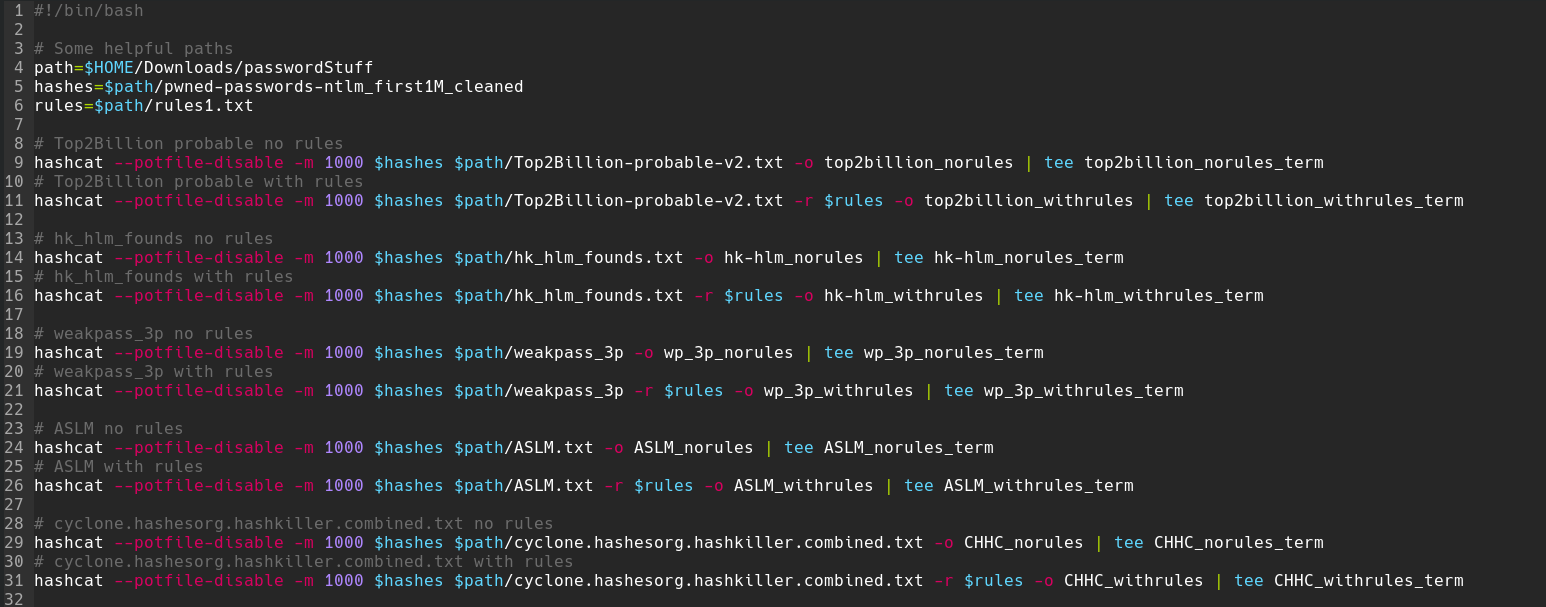
\includegraphics[width=\textwidth]{hashcatScript}}
\end{center}

\subsubsection{Results}
\begin{center}
\resizebox{\textwidth}{!}{%
\begin{tabular}{|p{10cm}|p{3cm}|p{2cm}|}
 \hline
 Dataset & Raw & Percent \\ [0.5ex] 
 \hline\hline
 Top2Billion-probable without rules & 245137/1000000 & 24.51\%\\
 \hline 
 Top2Billion-probable with rules & 369683/1000000 & 36.97\%\\
 \hline\hline
 hk-hlm-founds without rules & 28399/1000000 & 2.84\%\\
 \hline
 hk-hlm-founds with rules & 99867/1000000 & 9.99\%\\
 \hline\hline
 cyclone.hashesorg.hashkiller.combined without rules & 934087/1000000 & 93.41\%\\
 \hline
 cyclone.hashesorg.hashkiller.combined with rules & 934344/1000000 & 93.43\%\\
 \hline\hline
 weakpass-3p without rules & 55876/1000000 & 85.59\%\\
 \hline
 weakpass-3p with rules & 863702/1000000 & 86.37\%\\
 \hline\hline
 ASLM without rules & 52045/1000000 & 5.20\%\\
 \hline
 ASLM with rules & 150402/1000000 & 15.04\%\\
 \hline
\end{tabular}
}
\end{center}

\subsubsection{Password cracking analysis conclusion}
The cyclone.hashesorg.hashkiller.combined dataset achieved an incredibly high recovery rate, this indicates that pwned-passwords-ntlm-ordered-by-hash-v7 was probably made using this dataset, as 93\% recovery is not very realistic.
Pictured below are some of the ``passwords'' that the CHHC dataset managed to recover (hashes left of the \textbf{:}, ``passwords'' on the right), further solidifying the idea that the recovery rate is high not because of dataset realism, but because they overlap.
\begin{center}
\makebox[\textwidth]{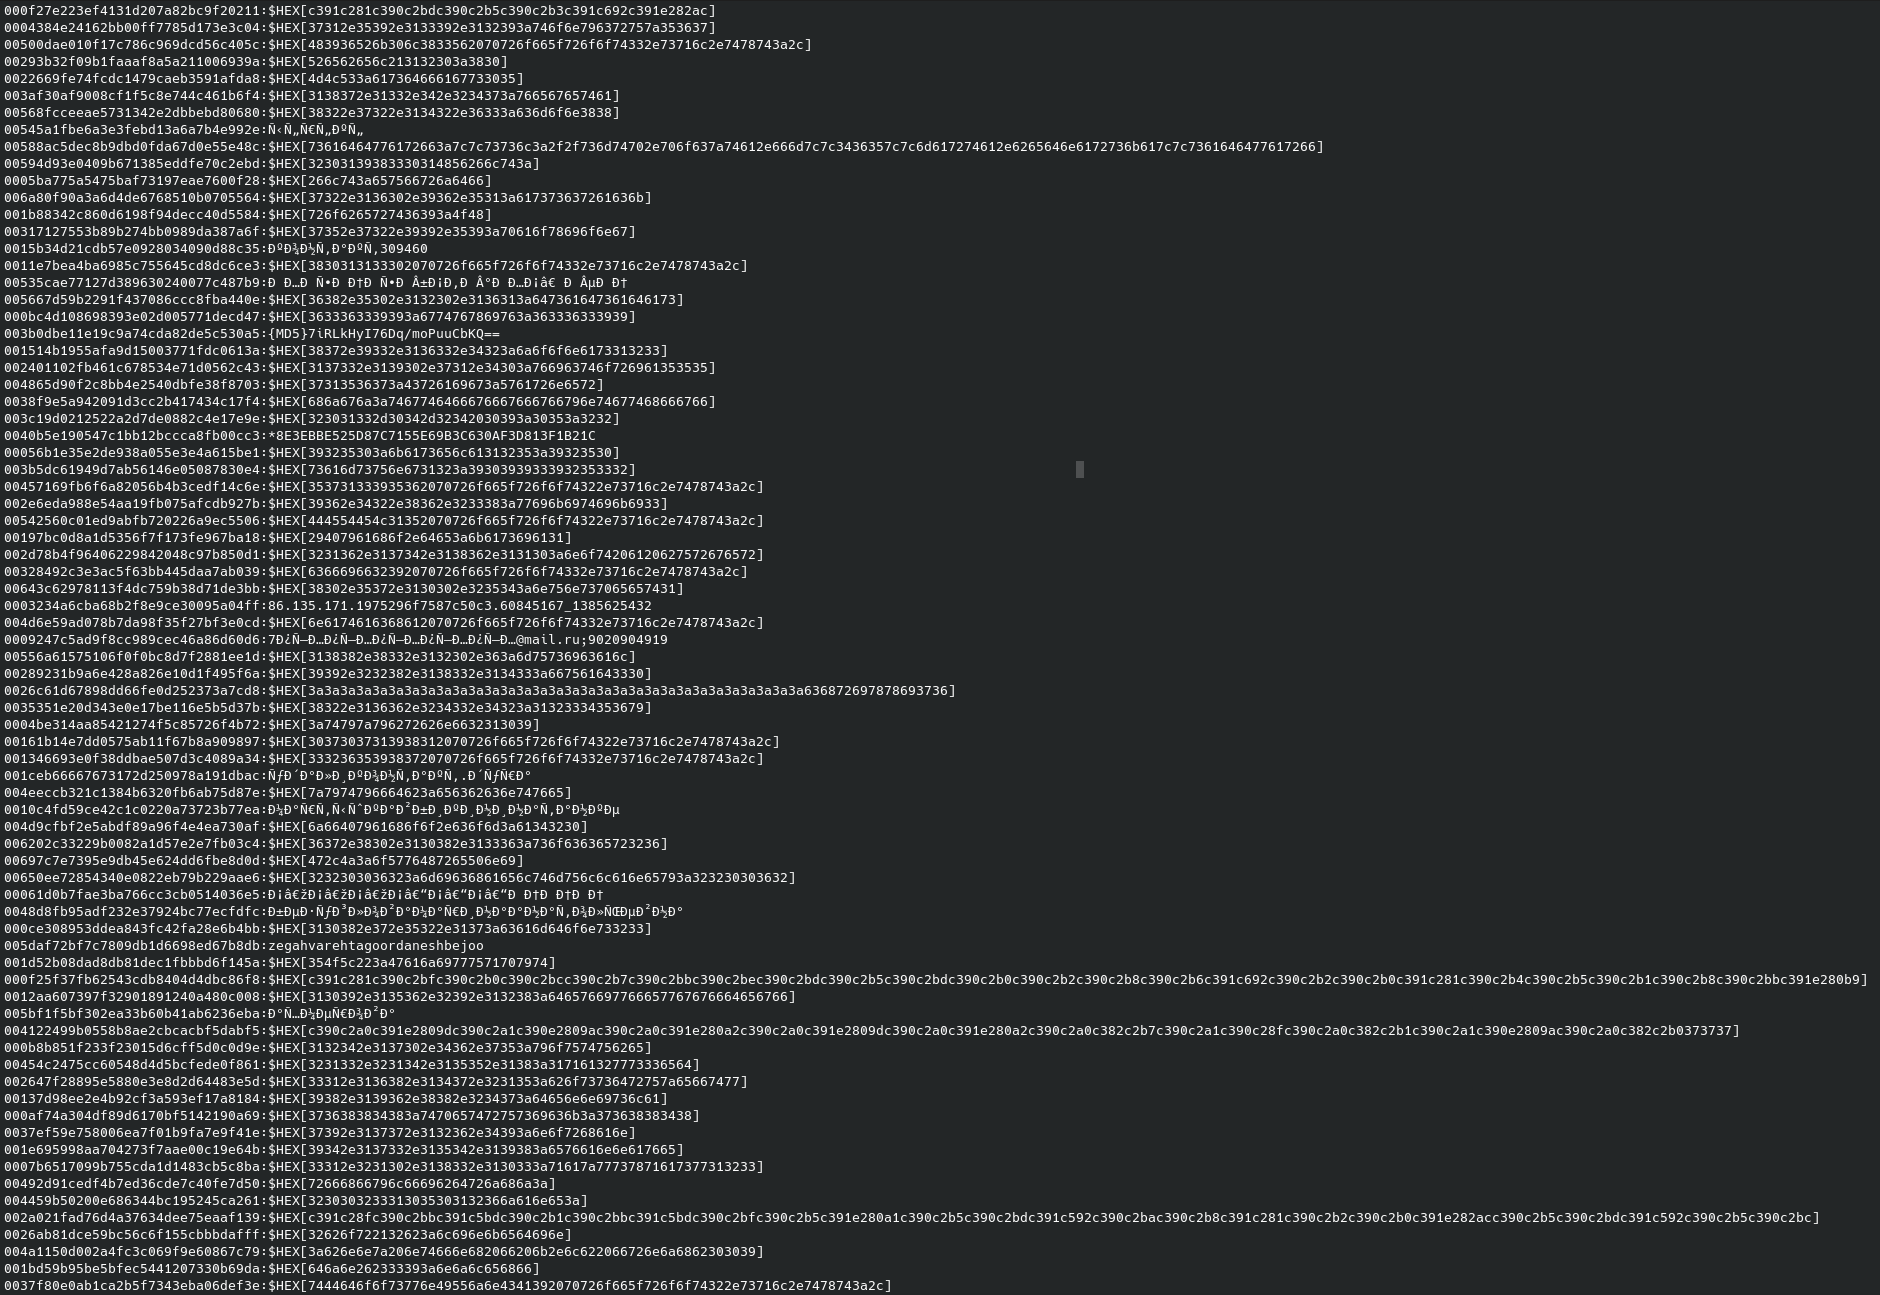
\includegraphics[width=10cm]{junkData}}
\end{center}
This demonstrates that my analysis of password cracking is in some sense flawed due to the datasets I am using.
Due to this apparent flaw in my methods, I cannot reliably come to any conclusions about the rate at which real-world passwords can be cracked using dictionary attacks.
If the time constraints of this project were not so strict, I could attempt to source a more reliable dataset of password hashes and retry this experiment.


\section{Vulnerabilities} \label{VULN}
A variety of vulnerabilities can be exploited to gain unauthorised access to a system which utilises passwords for authentication, these attacks can exploit technical flaws, human behaviour, or both.
\subsection{Human(user) vulnerabilities}
\subsubsection{Weak passwords and password behaviour}
One of the major problems with password-based authentication systems is that users are often quite lazy with their choice of passwords.
Choosing easily guessed passwords and re-using passwords are incredibly common.
This is often due to the large amount of misconceptions that users may have about password security.\\\\
``Addressing Misconceptions About Password Security Effectively'' \cite{mayer2018addressing} conducted a systematic literature review to determine the misconceptions the general public may have about password security, as well as how to address them. 
This work identified 23 misconceptions about password security, which where broken down into four categories, composition, handling, attacks and miscellaneous. The first two of these categories are most relevant to this section.
\begin{itemize}
\item \textbf{Composition:}\\
Users misunderstanding what a secure password is composed of is very common. There are many ways users may misunderstand how to compose a secure password, but the five outlined by \cite{mayer2018addressing} are:
\begin{itemize}
\item Adding numbers makes passwords automatically more difficult to guess.
\item Adding symbols makes passwords automatically more difficult to guess.
\item Adding uppercase letters makes passwords automatically more difficult to guess.
\item Replacing lowercase letters in the password with numbers, symbols, or uppercase letters makes the password more difficult to guess.
\item A word from another language than the your own mother tongue is a secure password.
\end{itemize}
\item \textbf{Handling:}\\
Users misunderstanding what behaviour puts the security of their accounts at risk is also common. There are many ways users may misunderstand how to securely protect their passwords, but the six outlined by \cite{mayer2018addressing} are:
\begin{itemize}
\item Reusing passwords is ok for secure passwords, but should be avoided for weak passwords.
\item Reusing is ok for more frequently used passwords.
\item Reusing passwords is better than writing them down.
\item Notes of passwords do not need to be particularly protected.
\item Passwords have to be changed frequently.
\item Storing passwords in the browser does not mean one is using a password manager.
\end{itemize}
\end{itemize}



\subsubsection{Phishing}
Phishing attacks are a form of social engineering which attempt to trick victims into handing sensitive information over to an attacker.
Attackers generally impersonate some other trusted entity when sending attacks to victims, quite often in the form of a link inside an email.\\\\
Phishing is a major attack technique used to capture victim passwords, this is done by creating a fake log-in page for some service and then making efforts to redirect users to the fake log-in page instead of the legitimate log-in page for that service. This is often done by sending the target an email prompting them to log in to their account for some reason or another, providing them with a malicious link which appears to be the legitimate page.\\\\
Phishing can be incredibly effective at obtaining the passwords of unsuspecting targets, these passwords can then be used by the attacker to falsely authenticate themselves and perform actions inside the victims account.
\cite{aleroud2017phishing}

\subsection{Technical vulnerabilities}
\subsubsection{SQL injection}
SQL injection is a type of attack which targets web database files, it takes advantage of websites which send user input into an SQL query without proper validation and cleaning.
SQL injection can be used to expose hashed passwords stored on a database. The attacker can then attempt to decrypt these hashed passwords to gain access to user accounts on the service.

\subsubsection{MITM}
\textbf{M}an-\textbf{I}n-\textbf{T}he-\textbf{M}iddle attacks exploit systems by capturing and/or modifying communications between two target parties.
A man-in-the-middle attack is performed how it sounds, a malicious party sits in-between two targets, intercepting their communications.
On very insecure systems attackers could simply capture plaintext or hashed passwords being communicated across the network, but generally more complex techniques are required to capture sensitive information such as passwords. A man in the middle who has the ability to modify traffic could in theory redirect targets to a phishing webpage when they try and visit certain legitimate sites.


\section{Mitigations} \label{MIT}
\subsection{Addressing password security misconceptions}
Mitigating the risk of bad password security practices from users is mostly a matter of education.
\cite{mayer2018addressing} provides explanations of the truth behind each of the identified misconceptions, they referred to these texts as ``intervention texts''.
The authors then performed a user study, this evaluation of the intervention texts consisted of:
\begin{enumerate}
\item A pre-treatment questionnaire measuring the prevalence of the different misconceptions in their participant sample.
\item the treatment using the intervention texts alongside information describing attacks on passwords and user accounts as well as respective defences.
\item a post-treatment questionnaire measuring the prevalence of the different misconceptions in their participant sample after having been exposed to the interventions as well as collecting basic demographics data.
\end{enumerate}
They concluded that their interventions could be used to effectively decrease the prevalence of many of the identified misconceptions.

\subsection{Phishing}
\cite{aleroud2017phishing} describes a variety of ways in which phishing can be detected:
\subsubsection{Machine learning}
Machine learning and data mining techniques can be utilised for detecting phishing, specifically:\\\\
\large{\textbf{Classification:}}\\
When using classification techniques, a model will be created that takes some input email/text and produces an output classifying it as either legitimate or phishing mail.\\\\
\large{\textbf{Clustering:}}\\
Clustering is used very similarly to classification, it partitions a set of instances into two clusters, phishing and legitimate. The objective of clustering is to group objects based on their similarities.\\\\
\large{\textbf{Anomaly detection:}}\\
An anomaly is a pattern in data which is not consistent with expected normal behaviour.
Anomaly detection can be applied to the detection of phishing, treating phishing as an outlier.
Phishing websites and mail typically demonstrate abnormal behaviour compared to their legitimate counterparts, this abnormal behaviour can be detected.\\\\
\large{\textbf{Text mining:}}\\
Text mining refers to utilising data mining and machine learning techniques to discover trends, patterns, and any other useful knowledge from a piece of text.
Text mining can be used to detect phishing attempts by analysing patterns in the contents of emails, instant messages, URLs, websites, and more.
\subsubsection{Human detection}
\large{\textbf{Increasing user awareness:}}\\
Since phishing primarily exploits a lack of security awareness in targets, increasing this awareness should help reduce the amount of successful phishing attacks taking place significantly.
A variety of factors affect a users security awareness, including:
\begin{itemize}
\item Security knowledge
\item Web experience
\item Computer self-efficacy
\item Disposition to trust
\item Perceived risk
\item Suspicion of humanity
\end{itemize}
The primary technique used to increase the likelihood of human users successfully detecting phishing attempts is training and education.
One form of this is sending users security notices embedded in emails with graphics and text explaining what phishing attacks are and how to detect them, along with any other relevant important information.\\\\
\large{\textbf{Involving users in identifying phishing material:}}\\
Users are expected to be able to manually identify new phishing attempts through participation in identifying legitimate and phishing material.
There are two approaches:
\begin{enumerate}
\item Manual authentication. This approach notifies users to identify suspicious behaviour linked to phishing themselves, reminding them that they must also make an effort to prevent phishing attacks from successfully taking place.
\item User voting. This is an interesting approach where a community database is created and users can submit suspected phishes, other users can then vote for whether these submissions are phishing or legitimate. This can also be used to create labelled datasets for the training of machine-learned detection systems.
\end{enumerate}
\subsubsection{Other phishing countermeasures}
\large{\textbf{Honeypots:}}\\
Honeypots are traps created to capture information about attackers. These traps do this by convincing attackers that they are real victims, then observing exactly how the attacker decides to proceed with their phishing attempts. The data collected from observing the attacker can be used when building attacker blacklist databases, and/or to discover and block suspicious domains.\\\\
\large{\textbf{Search engines:}}\\
Search engines can be combined with other techniques to detect phishing. Typically legitimate pages are indexed and assigned a rank by search engines, this rank will generally be reasonably high, especially for major websites. Phishing domains will generally rank very low on search engines, or not be indexed at all, this means search engines can be used to detect suspicious links.

\subsection{Injection}
% reminder: honey passwords
\subsection{MITM}


\section{Conclusion} \label{CONCL}


\bibliographystyle{plain}
\bibliography{References}

\end{document}
